% TikZ Figure: Topic Specialization Matrix (AG News)
% Usage: % TikZ Figure: Topic Specialization Matrix (AG News)
% Usage: % TikZ Figure: Topic Specialization Matrix (AG News)
% Usage: % TikZ Figure: Topic Specialization Matrix (AG News)
% Usage: \input{tikzfigs/fig_accuracy_per_topic.tex}
% Self-contained color definitions
\providecolor{oursblue}{RGB}{46,111,183}
\providecolor{boundorange}{RGB}{224,164,58}
\providecolor{vllmred}{RGB}{209,73,91}
\providecolor{basegray}{RGB}{154,164,174}
\providecolor{traingreen}{RGB}{89,161,79}
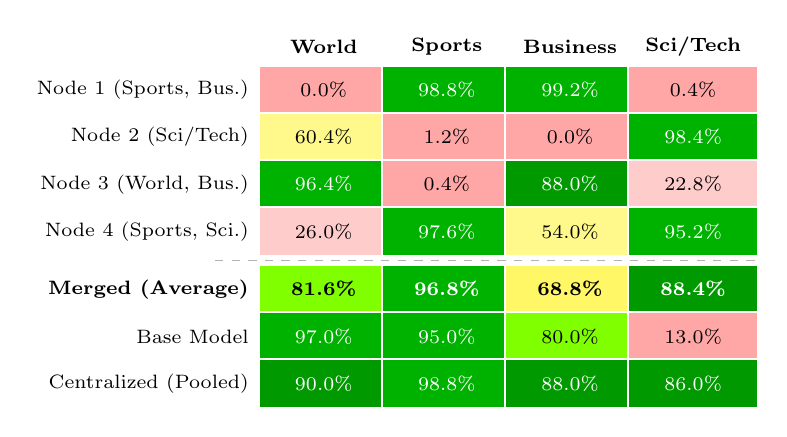
\begin{tikzpicture}[scale=0.92]
\tikzset{
    cell/.style={rectangle, minimum width=1.65cm, minimum height=0.62cm, draw=white, line width=0.8pt, font=\scriptsize, align=center},
    rowlabel/.style={font=\scriptsize, anchor=east, align=right},
    collabel/.style={font=\scriptsize\bfseries, align=center}
}

% Column Headers
\node[collabel] at (1.5, 0.6) {World};
\node[collabel] at (3.2, 0.6) {Sports};
\node[collabel] at (4.9, 0.6) {Business};
\node[collabel] at (6.6, 0.6) {Sci/Tech};

% Row 1: Node 1 (Sports, Business)
\node[rowlabel] at (0.6, 0.0) {Node 1 (Sports, Bus.)};
\node[cell, fill=red!35] at (1.5, 0.0) {0.0\%};
\node[cell, fill=green!70!black, text=white] at (3.2, 0.0) {98.8\%};
\node[cell, fill=green!70!black, text=white] at (4.9, 0.0) {99.2\%};
\node[cell, fill=red!35] at (6.6, 0.0) {0.4\%};

% Row 2: Node 2 (Sci/Tech)
\node[rowlabel] at (0.6, -0.65) {Node 2 (Sci/Tech)};
\node[cell, fill=yellow!45] at (1.5, -0.65) {60.4\%};
\node[cell, fill=red!35] at (3.2, -0.65) {1.2\%};
\node[cell, fill=red!35] at (4.9, -0.65) {0.0\%};
\node[cell, fill=green!70!black, text=white] at (6.6, -0.65) {98.4\%};

% Row 3: Node 3 (World, Business)
\node[rowlabel] at (0.6, -1.30) {Node 3 (World, Bus.)};
\node[cell, fill=green!70!black, text=white] at (1.5, -1.30) {96.4\%};
\node[cell, fill=red!35] at (3.2, -1.30) {0.4\%};
\node[cell, fill=green!60!black, text=white] at (4.9, -1.30) {88.0\%};
\node[cell, fill=red!20] at (6.6, -1.30) {22.8\%};

% Row 4: Node 4 (Sports, Sci/Tech)
\node[rowlabel] at (0.6, -1.95) {Node 4 (Sports, Sci.)};
\node[cell, fill=red!20] at (1.5, -1.95) {26.0\%};
\node[cell, fill=green!70!black, text=white] at (3.2, -1.95) {97.6\%};
\node[cell, fill=yellow!45] at (4.9, -1.95) {54.0\%};
\node[cell, fill=green!70!black, text=white] at (6.6, -1.95) {95.2\%};

% Separator line
\draw[gray!60, dashed, line width=0.5pt] (0.0, -2.35) -- (7.5, -2.35);

% Row 5: All Adapters Merged
\node[rowlabel] at (0.6, -2.75) {\bfseries Merged (Average)};
\node[cell, fill=green!50!yellow] at (1.5, -2.75) {\bfseries 81.6\%};
\node[cell, fill=green!70!black, text=white] at (3.2, -2.75) {\bfseries 96.8\%};
\node[cell, fill=yellow!60] at (4.9, -2.75) {\bfseries 68.8\%};
\node[cell, fill=green!60!black, text=white] at (6.6, -2.75) {\bfseries 88.4\%};

% Row 6: Base Model
\node[rowlabel] at (0.6, -3.40) {Base Model};
\node[cell, fill=green!70!black, text=white] at (1.5, -3.40) {97.0\%};
\node[cell, fill=green!70!black, text=white] at (3.2, -3.40) {95.0\%};
\node[cell, fill=green!50!yellow] at (4.9, -3.40) {80.0\%};
\node[cell, fill=red!35] at (6.6, -3.40) {13.0\%};

% Row 7: Centralized Training
\node[rowlabel] at (0.6, -4.05) {Centralized (Pooled)};
\node[cell, fill=green!60!black, text=white] at (1.5, -4.05) {90.0\%};
\node[cell, fill=green!70!black, text=white] at (3.2, -4.05) {98.8\%};
\node[cell, fill=green!60!black, text=white] at (4.9, -4.05) {88.0\%};
\node[cell, fill=green!60!black, text=white] at (6.6, -4.05) {86.0\%};

\end{tikzpicture}

% Self-contained color definitions
\providecolor{oursblue}{RGB}{46,111,183}
\providecolor{boundorange}{RGB}{224,164,58}
\providecolor{vllmred}{RGB}{209,73,91}
\providecolor{basegray}{RGB}{154,164,174}
\providecolor{traingreen}{RGB}{89,161,79}
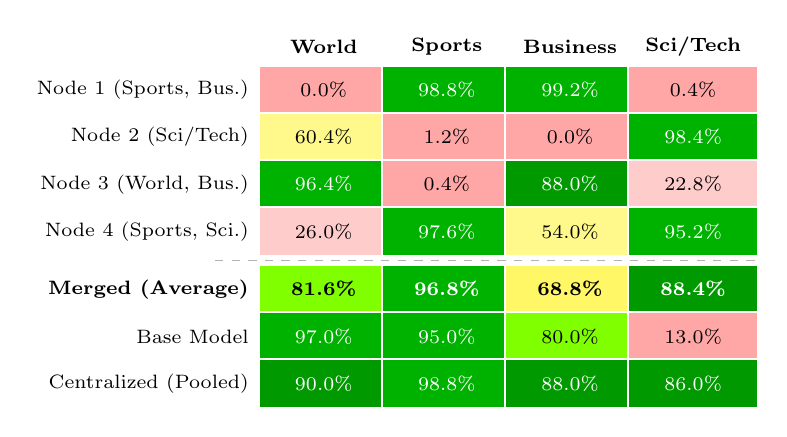
\begin{tikzpicture}[scale=0.92]
\tikzset{
    cell/.style={rectangle, minimum width=1.65cm, minimum height=0.62cm, draw=white, line width=0.8pt, font=\scriptsize, align=center},
    rowlabel/.style={font=\scriptsize, anchor=east, align=right},
    collabel/.style={font=\scriptsize\bfseries, align=center}
}

% Column Headers
\node[collabel] at (1.5, 0.6) {World};
\node[collabel] at (3.2, 0.6) {Sports};
\node[collabel] at (4.9, 0.6) {Business};
\node[collabel] at (6.6, 0.6) {Sci/Tech};

% Row 1: Node 1 (Sports, Business)
\node[rowlabel] at (0.6, 0.0) {Node 1 (Sports, Bus.)};
\node[cell, fill=red!35] at (1.5, 0.0) {0.0\%};
\node[cell, fill=green!70!black, text=white] at (3.2, 0.0) {98.8\%};
\node[cell, fill=green!70!black, text=white] at (4.9, 0.0) {99.2\%};
\node[cell, fill=red!35] at (6.6, 0.0) {0.4\%};

% Row 2: Node 2 (Sci/Tech)
\node[rowlabel] at (0.6, -0.65) {Node 2 (Sci/Tech)};
\node[cell, fill=yellow!45] at (1.5, -0.65) {60.4\%};
\node[cell, fill=red!35] at (3.2, -0.65) {1.2\%};
\node[cell, fill=red!35] at (4.9, -0.65) {0.0\%};
\node[cell, fill=green!70!black, text=white] at (6.6, -0.65) {98.4\%};

% Row 3: Node 3 (World, Business)
\node[rowlabel] at (0.6, -1.30) {Node 3 (World, Bus.)};
\node[cell, fill=green!70!black, text=white] at (1.5, -1.30) {96.4\%};
\node[cell, fill=red!35] at (3.2, -1.30) {0.4\%};
\node[cell, fill=green!60!black, text=white] at (4.9, -1.30) {88.0\%};
\node[cell, fill=red!20] at (6.6, -1.30) {22.8\%};

% Row 4: Node 4 (Sports, Sci/Tech)
\node[rowlabel] at (0.6, -1.95) {Node 4 (Sports, Sci.)};
\node[cell, fill=red!20] at (1.5, -1.95) {26.0\%};
\node[cell, fill=green!70!black, text=white] at (3.2, -1.95) {97.6\%};
\node[cell, fill=yellow!45] at (4.9, -1.95) {54.0\%};
\node[cell, fill=green!70!black, text=white] at (6.6, -1.95) {95.2\%};

% Separator line
\draw[gray!60, dashed, line width=0.5pt] (0.0, -2.35) -- (7.5, -2.35);

% Row 5: All Adapters Merged
\node[rowlabel] at (0.6, -2.75) {\bfseries Merged (Average)};
\node[cell, fill=green!50!yellow] at (1.5, -2.75) {\bfseries 81.6\%};
\node[cell, fill=green!70!black, text=white] at (3.2, -2.75) {\bfseries 96.8\%};
\node[cell, fill=yellow!60] at (4.9, -2.75) {\bfseries 68.8\%};
\node[cell, fill=green!60!black, text=white] at (6.6, -2.75) {\bfseries 88.4\%};

% Row 6: Base Model
\node[rowlabel] at (0.6, -3.40) {Base Model};
\node[cell, fill=green!70!black, text=white] at (1.5, -3.40) {97.0\%};
\node[cell, fill=green!70!black, text=white] at (3.2, -3.40) {95.0\%};
\node[cell, fill=green!50!yellow] at (4.9, -3.40) {80.0\%};
\node[cell, fill=red!35] at (6.6, -3.40) {13.0\%};

% Row 7: Centralized Training
\node[rowlabel] at (0.6, -4.05) {Centralized (Pooled)};
\node[cell, fill=green!60!black, text=white] at (1.5, -4.05) {90.0\%};
\node[cell, fill=green!70!black, text=white] at (3.2, -4.05) {98.8\%};
\node[cell, fill=green!60!black, text=white] at (4.9, -4.05) {88.0\%};
\node[cell, fill=green!60!black, text=white] at (6.6, -4.05) {86.0\%};

\end{tikzpicture}

% Self-contained color definitions
\providecolor{oursblue}{RGB}{46,111,183}
\providecolor{boundorange}{RGB}{224,164,58}
\providecolor{vllmred}{RGB}{209,73,91}
\providecolor{basegray}{RGB}{154,164,174}
\providecolor{traingreen}{RGB}{89,161,79}
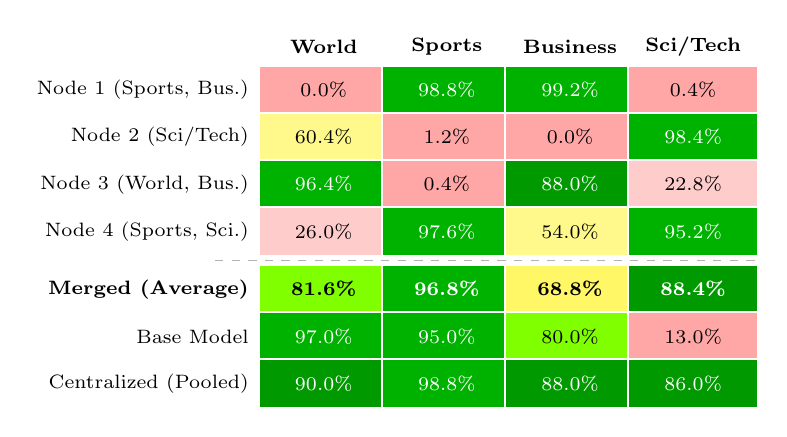
\begin{tikzpicture}[scale=0.92]
\tikzset{
    cell/.style={rectangle, minimum width=1.65cm, minimum height=0.62cm, draw=white, line width=0.8pt, font=\scriptsize, align=center},
    rowlabel/.style={font=\scriptsize, anchor=east, align=right},
    collabel/.style={font=\scriptsize\bfseries, align=center}
}

% Column Headers
\node[collabel] at (1.5, 0.6) {World};
\node[collabel] at (3.2, 0.6) {Sports};
\node[collabel] at (4.9, 0.6) {Business};
\node[collabel] at (6.6, 0.6) {Sci/Tech};

% Row 1: Node 1 (Sports, Business)
\node[rowlabel] at (0.6, 0.0) {Node 1 (Sports, Bus.)};
\node[cell, fill=red!35] at (1.5, 0.0) {0.0\%};
\node[cell, fill=green!70!black, text=white] at (3.2, 0.0) {98.8\%};
\node[cell, fill=green!70!black, text=white] at (4.9, 0.0) {99.2\%};
\node[cell, fill=red!35] at (6.6, 0.0) {0.4\%};

% Row 2: Node 2 (Sci/Tech)
\node[rowlabel] at (0.6, -0.65) {Node 2 (Sci/Tech)};
\node[cell, fill=yellow!45] at (1.5, -0.65) {60.4\%};
\node[cell, fill=red!35] at (3.2, -0.65) {1.2\%};
\node[cell, fill=red!35] at (4.9, -0.65) {0.0\%};
\node[cell, fill=green!70!black, text=white] at (6.6, -0.65) {98.4\%};

% Row 3: Node 3 (World, Business)
\node[rowlabel] at (0.6, -1.30) {Node 3 (World, Bus.)};
\node[cell, fill=green!70!black, text=white] at (1.5, -1.30) {96.4\%};
\node[cell, fill=red!35] at (3.2, -1.30) {0.4\%};
\node[cell, fill=green!60!black, text=white] at (4.9, -1.30) {88.0\%};
\node[cell, fill=red!20] at (6.6, -1.30) {22.8\%};

% Row 4: Node 4 (Sports, Sci/Tech)
\node[rowlabel] at (0.6, -1.95) {Node 4 (Sports, Sci.)};
\node[cell, fill=red!20] at (1.5, -1.95) {26.0\%};
\node[cell, fill=green!70!black, text=white] at (3.2, -1.95) {97.6\%};
\node[cell, fill=yellow!45] at (4.9, -1.95) {54.0\%};
\node[cell, fill=green!70!black, text=white] at (6.6, -1.95) {95.2\%};

% Separator line
\draw[gray!60, dashed, line width=0.5pt] (0.0, -2.35) -- (7.5, -2.35);

% Row 5: All Adapters Merged
\node[rowlabel] at (0.6, -2.75) {\bfseries Merged (Average)};
\node[cell, fill=green!50!yellow] at (1.5, -2.75) {\bfseries 81.6\%};
\node[cell, fill=green!70!black, text=white] at (3.2, -2.75) {\bfseries 96.8\%};
\node[cell, fill=yellow!60] at (4.9, -2.75) {\bfseries 68.8\%};
\node[cell, fill=green!60!black, text=white] at (6.6, -2.75) {\bfseries 88.4\%};

% Row 6: Base Model
\node[rowlabel] at (0.6, -3.40) {Base Model};
\node[cell, fill=green!70!black, text=white] at (1.5, -3.40) {97.0\%};
\node[cell, fill=green!70!black, text=white] at (3.2, -3.40) {95.0\%};
\node[cell, fill=green!50!yellow] at (4.9, -3.40) {80.0\%};
\node[cell, fill=red!35] at (6.6, -3.40) {13.0\%};

% Row 7: Centralized Training
\node[rowlabel] at (0.6, -4.05) {Centralized (Pooled)};
\node[cell, fill=green!60!black, text=white] at (1.5, -4.05) {90.0\%};
\node[cell, fill=green!70!black, text=white] at (3.2, -4.05) {98.8\%};
\node[cell, fill=green!60!black, text=white] at (4.9, -4.05) {88.0\%};
\node[cell, fill=green!60!black, text=white] at (6.6, -4.05) {86.0\%};

\end{tikzpicture}

% Self-contained color definitions
\providecolor{oursblue}{RGB}{46,111,183}
\providecolor{boundorange}{RGB}{224,164,58}
\providecolor{vllmred}{RGB}{209,73,91}
\providecolor{basegray}{RGB}{154,164,174}
\providecolor{traingreen}{RGB}{89,161,79}
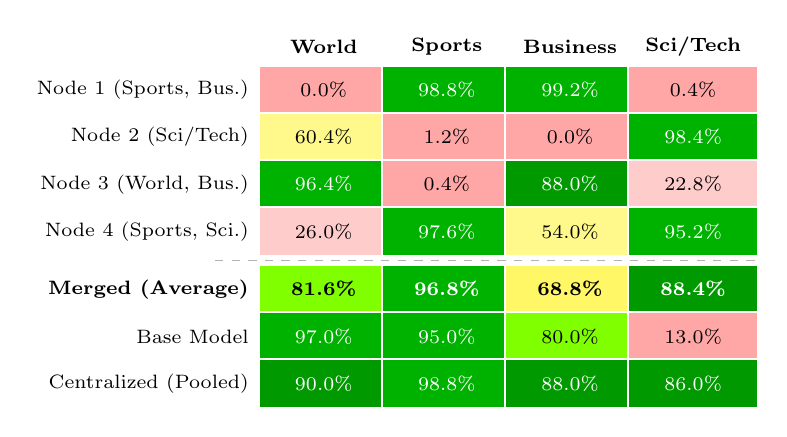
\begin{tikzpicture}[scale=0.92]
\tikzset{
    cell/.style={rectangle, minimum width=1.65cm, minimum height=0.62cm, draw=white, line width=0.8pt, font=\scriptsize, align=center},
    rowlabel/.style={font=\scriptsize, anchor=east, align=right},
    collabel/.style={font=\scriptsize\bfseries, align=center}
}

% Column Headers
\node[collabel] at (1.5, 0.6) {World};
\node[collabel] at (3.2, 0.6) {Sports};
\node[collabel] at (4.9, 0.6) {Business};
\node[collabel] at (6.6, 0.6) {Sci/Tech};

% Row 1: Node 1 (Sports, Business)
\node[rowlabel] at (0.6, 0.0) {Node 1 (Sports, Bus.)};
\node[cell, fill=red!35] at (1.5, 0.0) {0.0\%};
\node[cell, fill=green!70!black, text=white] at (3.2, 0.0) {98.8\%};
\node[cell, fill=green!70!black, text=white] at (4.9, 0.0) {99.2\%};
\node[cell, fill=red!35] at (6.6, 0.0) {0.4\%};

% Row 2: Node 2 (Sci/Tech)
\node[rowlabel] at (0.6, -0.65) {Node 2 (Sci/Tech)};
\node[cell, fill=yellow!45] at (1.5, -0.65) {60.4\%};
\node[cell, fill=red!35] at (3.2, -0.65) {1.2\%};
\node[cell, fill=red!35] at (4.9, -0.65) {0.0\%};
\node[cell, fill=green!70!black, text=white] at (6.6, -0.65) {98.4\%};

% Row 3: Node 3 (World, Business)
\node[rowlabel] at (0.6, -1.30) {Node 3 (World, Bus.)};
\node[cell, fill=green!70!black, text=white] at (1.5, -1.30) {96.4\%};
\node[cell, fill=red!35] at (3.2, -1.30) {0.4\%};
\node[cell, fill=green!60!black, text=white] at (4.9, -1.30) {88.0\%};
\node[cell, fill=red!20] at (6.6, -1.30) {22.8\%};

% Row 4: Node 4 (Sports, Sci/Tech)
\node[rowlabel] at (0.6, -1.95) {Node 4 (Sports, Sci.)};
\node[cell, fill=red!20] at (1.5, -1.95) {26.0\%};
\node[cell, fill=green!70!black, text=white] at (3.2, -1.95) {97.6\%};
\node[cell, fill=yellow!45] at (4.9, -1.95) {54.0\%};
\node[cell, fill=green!70!black, text=white] at (6.6, -1.95) {95.2\%};

% Separator line
\draw[gray!60, dashed, line width=0.5pt] (0.0, -2.35) -- (7.5, -2.35);

% Row 5: All Adapters Merged
\node[rowlabel] at (0.6, -2.75) {\bfseries Merged (Average)};
\node[cell, fill=green!50!yellow] at (1.5, -2.75) {\bfseries 81.6\%};
\node[cell, fill=green!70!black, text=white] at (3.2, -2.75) {\bfseries 96.8\%};
\node[cell, fill=yellow!60] at (4.9, -2.75) {\bfseries 68.8\%};
\node[cell, fill=green!60!black, text=white] at (6.6, -2.75) {\bfseries 88.4\%};

% Row 6: Base Model
\node[rowlabel] at (0.6, -3.40) {Base Model};
\node[cell, fill=green!70!black, text=white] at (1.5, -3.40) {97.0\%};
\node[cell, fill=green!70!black, text=white] at (3.2, -3.40) {95.0\%};
\node[cell, fill=green!50!yellow] at (4.9, -3.40) {80.0\%};
\node[cell, fill=red!35] at (6.6, -3.40) {13.0\%};

% Row 7: Centralized Training
\node[rowlabel] at (0.6, -4.05) {Centralized (Pooled)};
\node[cell, fill=green!60!black, text=white] at (1.5, -4.05) {90.0\%};
\node[cell, fill=green!70!black, text=white] at (3.2, -4.05) {98.8\%};
\node[cell, fill=green!60!black, text=white] at (4.9, -4.05) {88.0\%};
\node[cell, fill=green!60!black, text=white] at (6.6, -4.05) {86.0\%};

\end{tikzpicture}
